\begin{figure}[H]
    \centering
    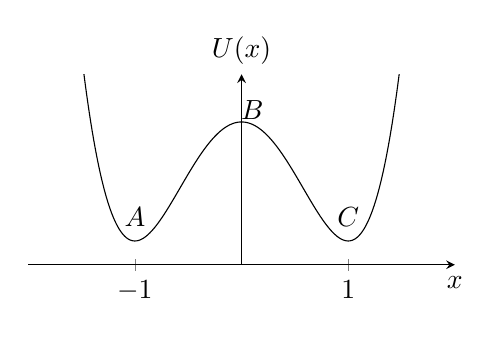
\begin{tikzpicture}
	\begin{axis}[
	    width=7cm,
	    height=4cm,
	    xmin= -2, xmax= 2,
	    ymin= 0, ymax = 0.4,
	    axis lines = middle,
	    x label style={at={(axis description cs:1,-0.01)},anchor=north},
	    y label style={at={(axis description cs:0.5,1)},anchor=south},
	    xlabel={$x$},
	    ylabel={$U(x)$ },
	    xtick={0, 1, -1},
	    xticklabels={$0$, $1$, $-1$},
	    ytick={0},
	    yticklabel={$0$},
	    ]
	    \addplot[domain=-3:3, samples=500]{-x^2/2*(1-x^2/2) + 0.3};
	    \node (C) [mark=dot] at (axis cs: 1, 0.1) {$C$};
	    \node (B) [mark=dot] at (axis cs: 0.1, 0.325) {$B$};
	    \node (A) [mark=dot] at (axis cs: -1, 0.1) {$A$};
	\end{axis}
    \end{tikzpicture}
    \begin{tikzpicture}
	\begin{axis}[
	    width=7cm,
	    height=4cm,
	    xmin= -2, xmax= 2,
	    ymin= -0.4, ymax = 0.4,
	    axis lines = middle,
	    x label style={at={(axis description cs:1,0.49)},anchor=north},
	    y label style={at={(axis description cs:0.5,1)},anchor=south},
	    xlabel={$x$},
	    ylabel={$U'(x)$ },
	    xtick={0, 1, -1},
	    xticklabels={$0$, $1$, $-1$},
	    ytick={0},
	    yticklabel={$0$},
	    ]
	    \addplot[domain=-3:3, samples=500]{-x+x^3};
	\end{axis}
    \end{tikzpicture}
    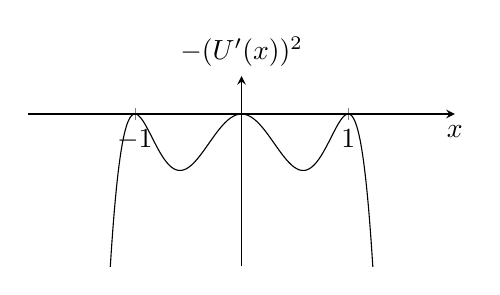
\begin{tikzpicture}
	\begin{axis}[
	    width=7cm,
	    height=4cm,
	    xmin= -2, xmax= 2,
	    ymin= -0.4, ymax = 0.1,
	    axis lines = middle,
	    x label style={at={(axis description cs:1,0.79)},anchor=north},
	    y label style={at={(axis description cs:0.5,1)},anchor=south},
	    xlabel={$x$},
	    ylabel={$-(U'(x))^2$ },
	    xtick={0, 1, -1},
	    xticklabels={$0$, $1$, $-1$},
	    ytick={0},
	    yticklabel={$0$},
	    ]
	    \addplot[domain=-2:2, samples=500]{-1*(-x+x^3)^2};
	\end{axis}
    \end{tikzpicture}
    \caption{\scriptsize Potenziale in cui vivono i camminatori e la sua derivata strettamente legata alla forza sul camminatore.}
    \label{fig:12_pot_der}
\end{figure}
